\documentclass{standalone}
\usepackage{tikz}
\usetikzlibrary{positioning, shapes.geometric, calc}  % <--- NEU: calc dazu!

\begin{document}

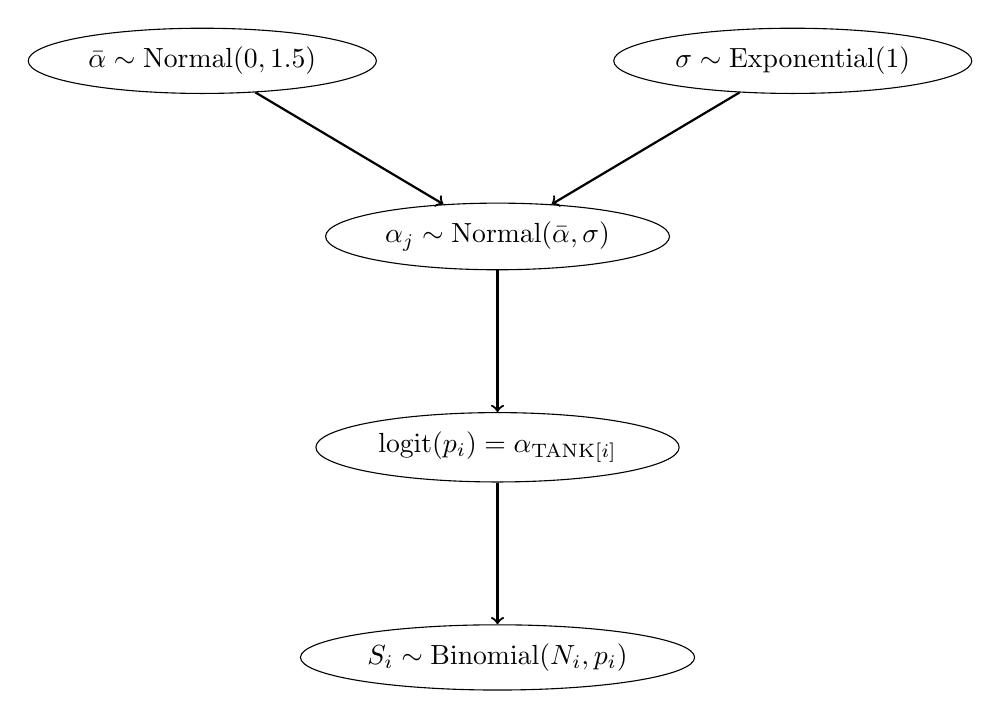
\begin{tikzpicture}[
    node distance=1.8cm and 3cm,
    every node/.style={draw, ellipse, align=center, minimum width=3.5cm, font=\normalsize}
]

% Nodes
\node (bar_alpha) {\(\bar{\alpha} \sim \mathrm{Normal}(0, 1.5)\)};
\node (sigma) [right=of bar_alpha] {\(\sigma \sim \mathrm{Exponential}(1)\)};
\node (alpha_j) [below=of $(bar_alpha)!0.5!(sigma)$] {\(\alpha_j \sim \mathrm{Normal}(\bar{\alpha}, \sigma)\)};
\node (pi) [below=of alpha_j] {\(\mathrm{logit}(p_i) = \alpha_{\mathrm{TANK}[i]}\)};
\node (Si) [below=of pi] {\(S_i \sim \mathrm{Binomial}(N_i, p_i)\)};

% Arrows
\draw[->, thick] (bar_alpha) -- (alpha_j);
\draw[->, thick] (sigma) -- (alpha_j);
\draw[->, thick] (alpha_j) -- (pi);
\draw[->, thick] (pi) -- (Si);

\end{tikzpicture}

\end{document}